%% LyX 2.3.6.1 created this file.  For more info, see http://www.lyx.org/.
%% Do not edit unless you really know what you are doing.
\documentclass[english]{article}
\usepackage[T1]{fontenc}
\usepackage[latin9]{inputenc}
\usepackage{geometry}
\geometry{verbose,tmargin=2.5cm,bmargin=2.5cm,lmargin=2.5cm,rmargin=2.5cm}
\usepackage{array}
\usepackage{calc}
\usepackage{textcomp}
\usepackage{multirow}
\usepackage{amsmath}
\usepackage{graphicx}

\makeatletter

%%%%%%%%%%%%%%%%%%%%%%%%%%%%%% LyX specific LaTeX commands.
%% Because html converters don't know tabularnewline
\providecommand{\tabularnewline}{\\}

\makeatother

\usepackage{babel}
\begin{document}
{[}SPLIT\_HERE{]}
\begin{enumerate}
\item \textbf{{[}JPJC/PRELIM/9597/2019/P1/Q1{]} }

The file \texttt{VISITORS.txt} contains the number of visitors to
Singapore from 1978 to 2018. Each line of the text file is in the
following format: 
\noindent \begin{center}
\texttt{<year>,<month>,<number\_of\_visitors> }
\par\end{center}

\subsection*{Task 1.1 }

Write program code to 
\begin{itemize}
\item read the data from the file and store them in an appropriate data
structure, 
\item get user input to select the \textbf{year(s)} to display for \textbf{total
number of visitors}, 
\item ensure that user input for\textbf{ start year} and \textbf{end year}
are valid, 
\item display the \textbf{year(s)} and \textbf{number of visitors}. 
\end{itemize}
Sample output: 

\noindent\fbox{\begin{minipage}[t]{1\columnwidth - 2\fboxsep - 2\fboxrule}%
\texttt{Start year : 1978}

\texttt{End year ~~: 1980}

\texttt{Year Number of visitors }

\texttt{1978 1234567 }

\texttt{1979 1542384 }

\texttt{1980 1278652 }%
\end{minipage}}

\subsection*{Evidence 1 }

Your program code. \hfill{}{[}11{]}

\subsection*{Task 1.2 }

Test your program with \textbf{four} relevant test data for user input.
Copy the table with the following headings to show your test cases. 
\noindent \begin{center}
\begin{tabular}{|c|c|c|}
\hline 
Test data & Purpose of test data & Expected results \tabularnewline
\hline 
 &  & \tabularnewline
\hline 
\end{tabular} 
\par\end{center}

\subsection*{Evidence 2 }

Completed table with \textbf{four} test cases. 

Screenshots of running your program with the \textbf{four} test cases.
\hfill{}{[}4{]}

{[}SPLIT\_HERE{]}
\item \textbf{{[}JPJC/PRELIM/9597/2019/P1/Q2{]} }

The incomplete pseudocode function below takes in an array as input.
The array will then be sorted in ascending order and the results will
be returned. Note that the start index of the array is 1. 

\noindent %
\noindent\begin{minipage}[t]{1\columnwidth}%
\texttt{FUNCTION SomeSort(SomeList : ARRAY) }

\texttt{\qquad{}FOR Pointer \textleftarrow{} 2 TO NumberOfItems }

\texttt{\qquad{}\qquad{}ItemToBeInserted \textleftarrow{} SomeList{[}Pointer{]} }

\texttt{\qquad{}\qquad{}CurrentItem \textleftarrow{} Pointer \textendash{}
1 }

\texttt{\qquad{}\qquad{}WHILE(SomeList{[}CurrentItem{]}>ItemToBeInserted
AND CurrentItem>0) }

\texttt{\qquad{}\qquad{}\qquad{}SomeList{[}CurrentItem+1{]} \textleftarrow{}
SomeList{[}CurrentItem{]} }

\texttt{\qquad{}\qquad{}\qquad{}CurrentItem \textleftarrow{} CurrentItem
- 1 }

\texttt{\qquad{}\qquad{}ENDWHILE}

\texttt{\qquad{}\qquad{}............... $\mathtt{A}$............... }

\texttt{\qquad{}ENDFOR }

\texttt{\qquad{}RETURN ARRAY}

\texttt{ENDFUNCTION }%
\end{minipage}

\subsection*{Task 2.1 }

Complete the missing line and write program code to implement the
complete function. Sort the array given in the file \texttt{NUMBERS.txt}.
You may copy and paste the array into your program code. 

\subsection*{Evidence 3 }
\begin{itemize}
\item Your program code. 
\item Screenshot showing the array before and after running the function.\hfill{}
{[}7{]}
\end{itemize}

\subsection*{Task 2.2 }

Write a bubble sort function that takes an array, sorts the array
and returns the array. 

\subsection*{Evidence 4 }

Your bubble sort function.\hfill{} {[}4{]}

\subsection*{Task 2.3 }

Amend your program code in both functions to count and display the
number of comparisons made when sorting the array. 

\subsection*{Evidence 5 }
\begin{itemize}
\item Your amended program code. 
\item Screenshot of running both sorting functions with number of comparisons
displayed.\hfill{} {[}4{]}
\end{itemize}
{[}SPLIT\_HERE{]}
\item \textbf{{[}JPJC/PRELIM/9597/2019/P1/Q3{]} }

JP Medical Centre uses a priority queue to register patients who visit
for medical attention. Upon registration at the medical centre, each
patient will be assigned a priority number according to the urgency
in seeking medical care. The urgent cases receive top priority and
go directly to the front of the queue, whereas the minor cases are
added to the bottom of the queue.

A priority queue is an extension of queue with the following properties.
\begin{itemize}
\item Every element has a priority associated with it. Higher priority has
a larger number. 
\item An element with high priority leaves the queue before an element with
low priority.
\item If two elements have the same priority, they are served according
to their order in the queue, i.e. the earlier element will be served
before the later element (FIFO). 
\end{itemize}
An example of operations on a priority queue is shown below:

\textbf{Initial state of priority queue} 

\begin{tabular}{|c|c|c|c|c|c|}
\hline 
Data & \textquoteleft jim\textquoteright{} & \textquoteleft ben\textquoteright{} & \textquoteleft ken\textquoteright{} & \textquoteleft wayne\textquoteright{} & \textquoteleft harry\textquoteright{}\tabularnewline
\hline 
Priority & 3 & 3 & 2 & 1 & 1\tabularnewline
\hline 
\multicolumn{1}{c}{} & \multicolumn{1}{c}{$\overset{\uparrow}{\boldsymbol{\text{front}}}$} & \multicolumn{1}{c}{} & \multicolumn{1}{c}{} & \multicolumn{1}{c}{} & \multicolumn{1}{c}{$\overset{\uparrow}{\boldsymbol{\text{rear}}}$}\tabularnewline
\end{tabular}

\textbf{Insert \textquoteleft jenny\textquoteright{} with priority
3:} \textquoteleft jenny\textquoteright{} joins the priority queue
ahead of \textquoteleft ken\textquoteright{} who has a priority of
2 

\begin{tabular}{|c|c|c|c|c|c|c|}
\hline 
Data & \textquoteleft jim\textquoteright{} & \textquoteleft ben\textquoteright{} & '\emph{jenny}' & \textquoteleft ken\textquoteright{} & \textquoteleft wayne\textquoteright{} & \textquoteleft harry\textquoteright{}\tabularnewline
\hline 
Priority & 3 & 3 & \emph{3} & 2 & 1 & 1\tabularnewline
\hline 
\multicolumn{1}{c}{} & \multicolumn{1}{c}{$\overset{\uparrow}{\boldsymbol{\text{front}}}$} & \multicolumn{1}{c}{} & \multicolumn{1}{c}{} & \multicolumn{1}{c}{} & \multicolumn{1}{c}{} & \multicolumn{1}{c}{$\overset{\uparrow}{\boldsymbol{\text{rear}}}$}\tabularnewline
\end{tabular}

Remove from priority queue: \textquoteleft jim\textquoteright{} is
removed from front of priority queue 

\begin{tabular}{|c|c|c|c|c|c|}
\hline 
Data & \textquoteleft ben\textquoteright{} & '\emph{jenny}' & \textquoteleft ken\textquoteright{} & \textquoteleft wayne\textquoteright{} & \textquoteleft harry\textquoteright{}\tabularnewline
\hline 
Priority & 3 & \emph{3} & 2 & 1 & 1\tabularnewline
\hline 
\multicolumn{1}{c}{} & \multicolumn{1}{c}{$\overset{\uparrow}{\boldsymbol{\text{front}}}$} & \multicolumn{1}{c}{} & \multicolumn{1}{c}{} & \multicolumn{1}{c}{} & \multicolumn{1}{c}{$\overset{\uparrow}{\boldsymbol{\text{rear}}}$}\tabularnewline
\end{tabular}

A \textbf{priority queue} abstract data type (ADT) is to be \textbf{implemented}
as \textbf{a linked list} using object-oriented programming. Two classes
\texttt{Node} and \texttt{PQueue} have been identified. 
\begin{center}
\begin{tabular}{|l|l|l|}
\hline 
\multicolumn{3}{|c|}{\texttt{Class: Node}}\tabularnewline
\hline 
\texttt{\textbf{\hspace{0.01\columnwidth}}}\textbf{Identifier} & \texttt{\textbf{\hspace{0.01\columnwidth}}}\textbf{Data Type} & \texttt{\textbf{\hspace{0.05\columnwidth}}}\textbf{Description}\tabularnewline
\hline 
\multicolumn{3}{|l|}{\textbf{Properties}}\tabularnewline
\hline 
\texttt{Data} & \texttt{STRING} & The node data\tabularnewline
\hline 
\texttt{Priority} & \texttt{INTEGER} & Indicates priority of node. Higher value has higher priority.\tabularnewline
\hline 
\texttt{Pointer} & \texttt{INTEGER} & Pointer to next node in queue.\tabularnewline
\hline 
\end{tabular}
\par\end{center}

\begin{center}
\begin{tabular}{|l|l|l|}
\hline 
\multicolumn{3}{|c|}{\texttt{Class: PQueue}}\tabularnewline
\hline 
\texttt{\textbf{\hspace{0.01\columnwidth}}}\textbf{Identifier} & \texttt{\textbf{\hspace{0.01\columnwidth}}}\textbf{Data Type} & \texttt{\textbf{\hspace{0.05\columnwidth}}}\textbf{Description}\tabularnewline
\hline 
\multicolumn{3}{|l|}{\textbf{Properties}}\tabularnewline
\hline 
\texttt{ThisPQueue} & \texttt{ARRAY{[}10{]} OF Node} & The data for the priority queue.\tabularnewline
\hline 
\texttt{Front} & \texttt{INTEGER} & Index for front node of queue. \tabularnewline
\hline 
\texttt{Rear} & \texttt{INTEGER} & Index for rear node of queue. \tabularnewline
\hline 
\texttt{NextFree} & \texttt{INTEGER} & Index for the next unused node.\tabularnewline
\hline 
\multicolumn{3}{|l|}{\textbf{Methods}}\tabularnewline
\hline 
\multirow{2}{*}{Initialise} & \multirow{2}{*}{\texttt{PROCEDURE}} & \textbullet{} Create a new priority queue \tabularnewline
 &  & \textbullet{} Initialise \texttt{Front} and \texttt{Rear} to -1.\tabularnewline
\hline 
\multirow{3}{*}{\texttt{JoinPQueue (NewItem:STRING, Priority:INTEGER)}} & \multirow{3}{*}{\texttt{PROCEDURE}} & \textbullet{} Create a new node of Node class.\tabularnewline
 &  & \textbullet{} Assign \texttt{NewItem} and \texttt{Priority} passed
as parameters to the \texttt{Data} and \texttt{Priority} attribute
of \texttt{Node}.\tabularnewline
 &  & \textbullet{} Assign \texttt{Node} to the \texttt{PQueue} according
to the priority of the node.\tabularnewline
\hline 
\multirow{2}{*}{\texttt{LeavePQueue}} & \multirow{2}{*}{\texttt{FUNCTION}} & \textbullet{} Remove \texttt{Node} from \texttt{PQueue}.\tabularnewline
 &  & \textbullet{} Return the \texttt{data} attribute of \texttt{Node}. \tabularnewline
\hline 
\end{tabular}
\par\end{center}

The diagram shows the linked list with: 
\begin{itemize}
\item the elements \textquoteleft ben\textquoteright , \textquoteleft jenny\textquoteright ,
\textquoteleft ken\textquoteright , \textquoteleft wayne\textquoteright ,
\textquoteleft harry\textquoteright{} in the priority queue
\item the unused nodes linked together
\end{itemize}
\begin{center}
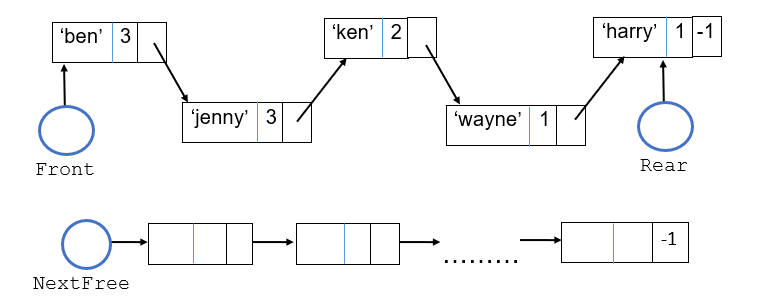
\includegraphics[width=0.65\paperwidth]{C:/Users/Admin/Desktop/Github/question_bank/LyX/static/img/9597-JPJC-2019-P1-Q3-1}
\par\end{center}

\subsection*{Task 3.1 }

Write program code to
\begin{itemize}
\item declare all the required identifiers for the \texttt{Node} and \texttt{PQueue}
class as specified, including the methods \texttt{Initialise}, \texttt{JoinPQueue},
\texttt{LeavePQueue}, and 
\item create the initial priority queue. 
\end{itemize}

\subsection*{Evidence 6: }

Your program code. \hfill{}{[}25{]}

\subsection*{Task 3.2 }

Write a procedure \texttt{OutputQueue} which displays the value of
\texttt{Front}, \texttt{Rear}, and \texttt{NextFree} and the contents
of \texttt{ThisPQueue} in index order. 

\subsection*{Evidence 7: }
\begin{itemize}
\item Your program code for \texttt{OutputPQueue}.
\item Screenshot for displaying the initial priority queue. \hfill{}{[}4{]}
\end{itemize}

\subsection*{Task 3.3 }

Write a main program to:
\begin{itemize}
\item Read from file\texttt{ PATIENTS.txt} all the data items with its priorities
into the priority queue by calling procedure \texttt{JoinPQueue}.
\item Output the priority queue by calling \texttt{OutputPQueue}. 
\end{itemize}

\subsection*{Evidence 8: }
\begin{itemize}
\item Your program code for task 3.3. 
\item Screenshot showing the output from running program in task 3.3. \hfill{}{[}5{]}
\end{itemize}
Task 3.4 

Write additional code in your main program that prints a menu with
the following options:

\noindent\fbox{\begin{minipage}[t]{1\columnwidth - 2\fboxsep - 2\fboxrule}%
\noindent \texttt{Patient Queue Menu }
\begin{enumerate}
\item[1)] \texttt{ Add patient to PQueue }
\item[2)] \texttt{ Remove patient from PQueue }
\item[3)] \texttt{ Display PQueue }
\item[4)] \texttt{ Exit program }
\end{enumerate}
%
\end{minipage}}

Write program code for each option by calling the appropriate methods
from the \texttt{PQueue} class. 

\subsection*{Evidence 9: }

Your program code for task 3.4.\hfill{} {[}4{]}

\subsection*{Task 3.5 }

Test your main program by doing the following in order and display
the priority queue: 
\noindent \begin{center}
\begin{tabular}{|l|l|l|l|}
\hline 
No. & Operation & Data  & Priority\tabularnewline
\hline 
1 & Remove patient & - & -\tabularnewline
\hline 
2 & Add patient & Donny & 2\tabularnewline
\hline 
\end{tabular} 
\par\end{center}

\subsection*{Evidence 10: }

Screenshot for testing your program in task 3.5.\hfill{} {[}2{]}

{[}SPLIT\_HERE{]}
\item \textbf{{[}JPJC/PRELIM/9597/2019/P1/Q4{]} }

You are to write a computer program to test the validity of classic
Sudoku puzzles. 

The classic Sudoku puzzle involves a grid of 81 squares. The grid
is divided into nine blocks, each containing nine squares. Each of
the nine blocks has to contain all the numbers 1 to 9 within its squares.
Each number can only appear once in a row, column or block. 

A $9\times9$ classic Sudoku puzzle can be represented using a two-dimensional
array. An example of this puzzle is:
\begin{center}
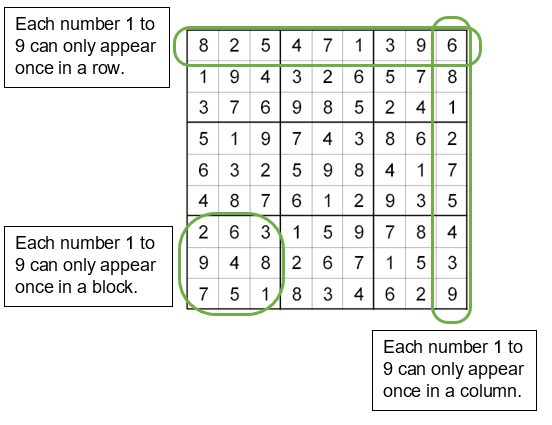
\includegraphics[width=0.5\paperwidth]{C:/Users/Admin/Desktop/Github/question_bank/LyX/static/img/9597-JPJC-2019-P1-Q4-1}
\par\end{center}

The puzzle can be displayed in this way on the computer. 
\noindent \begin{center}
\texttt{}%
\begin{tabular}{c}
\texttt{8 2 5 4 7 1 3 9 6}\tabularnewline
\texttt{1 9 4 3 2 6 5 7 8}\tabularnewline
\texttt{3 7 6 9 8 5 2 4 1}\tabularnewline
\texttt{5 1 9 7 4 3 8 6 2}\tabularnewline
\texttt{6 3 2 5 9 8 4 1 7}\tabularnewline
\texttt{4 8 7 6 1 2 9 3 5}\tabularnewline
\texttt{2 6 3 1 5 9 7 8 4}\tabularnewline
\texttt{9 4 8 2 6 7 1 5 3}\tabularnewline
\texttt{7 5 1 8 3 4 6 2 9}\tabularnewline
\end{tabular}
\par\end{center}

\noindent \begin{center}
\par\end{center}

\subsection*{Task 4.1 }

Write program code for a procedure \texttt{displayboard} that will
take a parameter \texttt{board} and display a puzzle declared as a
two-dimensional array. 

Copy and paste array \texttt{puzzle1} from the file \texttt{PUZZLES.txt}
into your program code. 

Call procedure \texttt{displayboard} to display \texttt{puzzle1}. 

\subsection*{Evidence 11: }
\begin{itemize}
\item Your program code for \texttt{displayboard} to display \texttt{puzzle1}. 
\item Screenshot of displaying \texttt{puzzle1} as a $9\times9$ Sudoku
puzzle.\hfill{} {[}5{]} 
\end{itemize}
To test the validity of a Sudoku puzzle, each of the rows, columns
and blocks can be checked to ensure that each number 1 to 9 only appears
once. 

\subsection*{Task 4.2 }

Write program code for a function \texttt{checkRow} that will check
all the nine rows of the puzzle to ensure that each number 1 to 9
only appears once. The function should take a parameter board and
return a Boolean value. 

\subsection*{Evidence 12: }

Your program code for \texttt{checkRow}.\hfill{} {[}6{]}

\subsection*{Task 4.3}

Write program code for a function \texttt{checkColumn} that will check
all the nine columns of the puzzle to ensure that each number 1 to
9 only appears once. The function should take a parameter \texttt{board}
and return a Boolean value.

\subsection*{Evidence 13: }

Your program code for \texttt{checkColumn}. \hfill{}{[}6{]}

\section*{Task 4.4 }

Write program code for a function \texttt{checkBlock} that will check
all the nine blocks of the puzzle to ensure that each number 1 to
9 only appear once. The function should take a parameter board and
return a Boolean value. 

\subsection*{Evidence 14: }

Your program code for \texttt{checkBlock}.\hfill{} {[}8{]}

\subsection*{Task 4.5 }

Write program code to call the three functions \texttt{checkrow},
\texttt{checkColumn}, and \texttt{checkBlock} to test the validity
of \texttt{puzzle1}, \texttt{puzzle2}, and \texttt{puzzle3} given
in the file \texttt{PUZZLES.txt}. Copy and paste these puzzles into
your program code. Your program should first display the puzzle before
printing statement(s) to show whether the puzzle is valid or not.
If invalid, state whether the invalidity is due to the row, column
or block.

\subsection*{Evidence 15:}

\textbullet{} Your program code for task 4.5 

\textbullet{} Screenshot of running task 4.5\hfill{} {[}5{]}

{[}SPLIT\_HERE{]}
\item \textbf{{[}JPJC/PRELIM/9597/2019/P2/Q1{]} }

Furniture retailer XFurniture is currently using a manual, paper-based
ordering system. 

The customer visits the show room and informs the salesperson his/her
furniture selection. After which, the salesperson asks the filing
clerk to locate the relevant paper files that contain all the necessary
details of the chosen item in the file cabinet. The files contain
the following information of a furniture item:
\begin{itemize}
\item item code 
\item description of item 
\item price of item 
\item delivery time 
\item details of the supplier
\end{itemize}
The customer pays for the purchase and the salesperson hands the original
purchase order, and a duplicate copy to the customer and the filing
clerk respectively. At the end of the day, the filing clerk will record
the total sales for the day and proceed to order the furniture from
the supplier by sending them a purchase order of the consolidated
furniture items sold for the day. 

The management of XFurniture decides to replace its current system
with a server--based ordering system. 

A system developer from an IT consultant firm is employed to carry
out the project. The first task is to write a project proposal. 
\begin{enumerate}
\item One section of the project proposal is the Problem Statement which
lists the problems in the current system. Write the Problem Statement.
\hfill{}{[}4{]}
\end{enumerate}
The system developer draws up a list of activities that will be required
for the completion of the software project:
\noindent \begin{center}
\begin{tabular}{|c|l|c|}
\hline 
Identifier & Activity & Estimated Duration (weeks)\tabularnewline
\hline 
A & Order and deliver the new database system and server & 4\tabularnewline
\hline 
B & Design and install the network infrastructure & 7\tabularnewline
\hline 
C & Order, deliver and install new PCs and printer & 9\tabularnewline
\hline 
D & est the database system, server and network & 3\tabularnewline
\hline 
E & Test the PCs with the server and network & 2\tabularnewline
\hline 
F & Copy existing sales data to the new database system & 1\tabularnewline
\hline 
G & Copy other existing PC software to the new PCs & 3\tabularnewline
\hline 
H & Test all software and database on the new PCs and server & 1\tabularnewline
\hline 
I & Train users & 2\tabularnewline
\hline 
\end{tabular}
\par\end{center}

Tasks A, B and C can be undertaken at the same time, but Task A and
Task B must be completed before Task D can commence. Tasks C and D
must be completed before Task E can begin. Task E must be completed
before Tasks F and G can start. Tasks F and G can be undertaken at
the same time, but both must be completed before Task H can commence.
Task I must follow Task H. 
\begin{enumerate}
\item[(b)]  Draw a PERT chart for this project. Provide a node key explaining
the layout and contents of the nodes used in your diagram. \hfill{}{[}4{]} 
\item[(c)]  Copy and complete the following table with the earliest and latest
start times, the earliest and latest finish times, duration, and float
time for each task. 
\noindent \begin{center}
\begin{tabular}{|c|c|c|c|c|c|c|}
\hline 
Task & EST & LST & EFT & LFT & Duration & Float\tabularnewline
\hline 
A & 0 & 3 & 4 & 7 & 4 & 3\tabularnewline
\hline 
B &  &  &  &  & 7 & \tabularnewline
\hline 
C &  &  &  &  & 9 & \tabularnewline
\hline 
D &  &  &  &  & 3 & \tabularnewline
\hline 
E &  &  &  &  & 2 & \tabularnewline
\hline 
F & 12 & 14 & 13 & 15 & 1 & \tabularnewline
\hline 
G &  &  &  &  & 3 & \tabularnewline
\hline 
H & 15 & 15 & 16 & 16 & 1 & \tabularnewline
\hline 
I & 16 & 16 & 18 & 18 & 2 & 0\tabularnewline
\hline 
\end{tabular} 
\par\end{center}

\hfill{}{[}4{]}
\item[(d)]  State the critical path.\hfill{} {[}1{]}
\item[(e)]  State the minimum time required for the project to be completed.
\hfill{} {[}1{]}
\item[(f)]  Dummy task may be used in PERT chart. What is a dummy task? \hfill{}
{[}1{]}
\item[(g)]  Draw a Gantt chart for the same project tasks, showing each of these
tasks, all dependencies, and the duration of each task. Highlight
the critical path on the Gantt chart.\hfill{} {[}4{]}
\end{enumerate}
{[}SPLIT\_HERE{]}
\item \textbf{{[}JPJC/PRELIM/9597/2019/P2/Q2{]} }

A project\textquoteright s software development life cycle includes
analysis, design, development, testing, implementation, and evaluation
stages.
\begin{enumerate}
\item Describe the following testing strategies that might be carried out
during a software development project, and explain how each type of
the testing strategy contributes to the overall quality of the project\textquoteright s
deliverables. 
\begin{enumerate}
\item Bottom-up testing. 
\item Top-down testing. \hfill{}{[}6{]}
\end{enumerate}
\item State two methods that could be used to implement a newly developed
system. Give a reason for each of the method chosen. \hfill{}{[}4{]}
\end{enumerate}
{[}SPLIT\_HERE{]}
\item \textbf{{[}JPJC/PRELIM/9597/2019/P2/Q3{]} }
\begin{enumerate}
\item \textbf{Copy} and \textbf{complete} the algorithm for a binary search
written in pseudocode shown below. It is given that the data being
searched is stored in the array \texttt{SearchData{[}63{]}}, and the
item of data being searched is stored in the variable \texttt{SearchItem}. 

\noindent %
\noindent\begin{minipage}[t]{1\columnwidth}%
\texttt{X <- 0 }

\texttt{Low <- 1 }

\texttt{High <- \dots \dots \dots \dots \dots \dots \dots \dots \dots \dots \dots \dots \dots \dots \dots{} }

\texttt{WHILE (High >= Low) AND (\dots \dots \dots \dots \dots \dots \dots \dots \dots \dots \dots \dots \dots \dots \dots \dots \dots \dots \dots )}

\texttt{\qquad{}Middle INT((High + Low)/2) }

\texttt{\qquad{}IF SearchData{[}Middle{]} = SearchItem }

\texttt{\qquad{}\qquad{}THEN }

\texttt{\qquad{}\qquad{}\qquad{}X <- Middle }

\texttt{\qquad{}\qquad{}ELSE}

\texttt{\qquad{}\qquad{}\qquad{}IF SearchData{[}Middle{]} < SearchItem }

\texttt{\qquad{}\qquad{}\qquad{}\qquad{}THEN}

\texttt{\qquad{}\qquad{}\qquad{}\qquad{}\qquad{}Low <- Middle
+ 1}

\texttt{\qquad{}\qquad{}\qquad{}\qquad{}ELSE }

\texttt{\qquad{}\qquad{}\qquad{}\qquad{}\qquad{}IF SearchData{[}Middle{]}
> SearchItem }

\texttt{\qquad{}\qquad{}\qquad{}\qquad{}\qquad{}\qquad{}THEN}

\texttt{\qquad{}\qquad{}\qquad{}\qquad{}\qquad{}\qquad{}\qquad{}\dots \dots \dots \dots \dots \dots \dots \dots \dots \dots \dots \dots \dots \dots \dots \dots{} }

\texttt{\qquad{}\qquad{}\qquad{}\qquad{}\qquad{}ENDIF }

\texttt{\qquad{}\qquad{}\qquad{}ENDIF }

\texttt{\qquad{}ENDIF }

\texttt{ENDWHILE }%
\end{minipage}

\hfill{}{[}3{]}
\item State the maximum number of comparisons that are required to find
an item which is present in \texttt{SearchData}. \hfill{} {[}1{]}
\item You will change the binary search algorithm to a recursive algorithm
and write the equivalent program code in the form of a procedure.
Name the recursive procedure \texttt{BinarySearch}. Use the following
variables: 
\noindent \begin{center}
\begin{tabular}{|l|l|l|}
\hline 
\textbf{Variable} & \textbf{Data Type} & \textbf{Description}\tabularnewline
\hline 
\texttt{SearchData} & \texttt{ARRAY{[}63{]} : INTEGER} & global array\tabularnewline
\hline 
\texttt{SearchItem} & \texttt{INTEGER} & global variable\tabularnewline
\hline 
\texttt{X} & \texttt{INTEGER} & global variable\tabularnewline
\hline 
\texttt{Low} & \texttt{INTEGER} & parameter\tabularnewline
\hline 
\texttt{High} & \texttt{INTEGER} & global variable\tabularnewline
\hline 
\texttt{Middle} & \texttt{INTEGER} & local variable\tabularnewline
\hline 
\end{tabular} 
\par\end{center}

Write pseudocode or program code for the recursive procedure \texttt{BinarySearch}.
\hfill{}{[}4{]}
\end{enumerate}
{[}SPLIT\_HERE{]}
\item \textbf{{[}JPJC/PRELIM/9597/2019/P2/Q4{]} }

Object-oriented programming is used to store and process data for
a company\textquoteright s payroll. 
\begin{center}
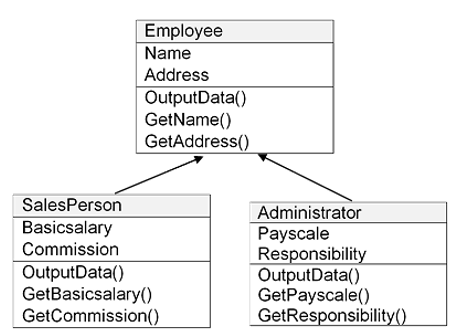
\includegraphics[width=0.5\paperwidth]{C:/Users/Admin/Desktop/Github/question_bank/LyX/static/img/9597-JPJC-2019-P2-Q4-1}
\par\end{center}
\begin{enumerate}
\item With reference to the class diagram shown above, explain: 
\begin{enumerate}
\item data encapsulation, and how classes support information hiding and
implementation independence. \hfill{}{[}3{]}
\item inheritance, and how it promotes software reusability. \hfill{}{[}2{]}
\end{enumerate}
\end{enumerate}
{[}SPLIT\_HERE{]}
\item \textbf{{[}JPJC/PRELIM/9597/2019/P2/Q5{]} }

With reference to \textbf{Question 1}, a server--based ordering system
will be implemented in XFurniture.

Local Area Network (LAN) will be used for the staff and customers.
\begin{enumerate}
\item Explain the meaning of a protocol for communication within the LAN.
\hfill{}{[}1{]}
\item State the purposes of switches and routers in a network. \hfill{}{[}4{]}
\item Explain the differences between using packet switching and circuit
switching in the transmission of a message. \hfill{} {[}3{]}
\item The LAN is connected to the Internet. Discuss the social and ethical
effects of allowing staff to have unrestricted access to the Internet.
\hfill{}{[}4{]}
\item Customers are now able to order furniture online after logging in
to the XFurniture online system. 
\begin{enumerate}
\item Explain why authentication techniques are necessary. \hfill{} {[}2{]}
\item Explain \textbf{two} methods for ensuring security of a network application.
\hfill{}{[}2{]}
\item A security policy is a formalised statement that defines how security
will be implemented within XFurniture. Explain why staff members are
required to know the need for privacy and integrity of data. \hfill{}{[}2{]}
\end{enumerate}
\item Explain why XFurniture has chosen to implement their server--based
ordering system over the intranet. \hfill{}{[}4{]}
\item An alternative to a server--based ordering system is to subscribe
the services of cloud computing. State the \textbf{three} services
provided by cloud computing, and explain how they can benefit XFurniture.
\hfill{} {[}6{]}
\end{enumerate}
{[}SPLIT\_HERE{]}
\item \textbf{{[}JPJC/PRELIM/9597/2019/P2/Q6{]} }

A reservation form used for booking JP Hotel rooms is shown:
\begin{center}
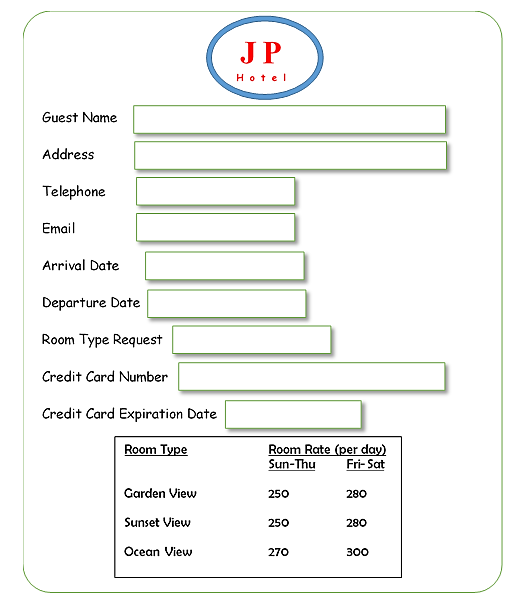
\includegraphics[width=0.5\paperwidth]{C:/Users/Admin/Desktop/Github/question_bank/LyX/static/img/9597-JPJC-2019-P2-Q6-1}
\par\end{center}

There are three room types available and the room rates are higher
for arrival on Fridays and Saturdays. A normalised database solution
is designed to store data for the hotel using a number of tables.
\begin{enumerate}
\item Draw an E-R diagram that shows these tables and the relationships
between them. \hfill{}{[}4{]}
\item Using standard notation, write the table descriptions of the tables
in part \textbf{(a)}. \hfill{} {[}6{]}
\end{enumerate}
To book a room in JP Hotel, the guest can fill in the hotel reservation
form with details specified on the form. After the form is submitted,
the credit card number and its expiration date are validated. The
guest will be notified with a message if the credit card number is
invalid. If the credit card number is valid, details of the guests
will be stored in a file. The room type requested by the guest will
then be checked for availability. If room type requested by guest
is available, a confirmation letter will be sent to the guest. 
\begin{enumerate}
\item[(c)]  Draw a data flow diagram for the hotel reservation system. \hfill{}{[}8{]}
\item[(d)]  A hotel room accommodates two guests and also includes breakfast
for two. The hotel allows for an additional guest to stay in a room
booked for two guests at a charge of \$80. An extra bed may be requested
for the additional guest at a charge of \$20. Breakfast can also be
provided for the additional guest at \$20.
\begin{enumerate}
\item Create a decision table showing all the possible conditions and actions.
\hfill{} {[}4{]}
\item Simplify your decision table by removing redundancies. \hfill{} {[}2{]}
\end{enumerate}
\end{enumerate}
{[}SPLIT\_HERE{]}
\item \textbf{{[}JPJC/PRELIM/9597/2019/P2/Q7{]} }
\begin{enumerate}
\item Computers use character codes that can be represented by ASCII and
Unicode. Explain the differences between these two character encoding
systems. \hfill{}{[}2{]}
\item Given that \textbf{two} bytes are used to represent a positive integer,
what is the denary number that corresponds to the \textbf{two} successive
bytes below? 
\noindent \begin{center}
\texttt{10010101 00110011} 
\par\end{center}

\noindent \begin{center}
\hfill{}\texttt{ }{[}2{]}
\par\end{center}
\item What is the hexadecimal number of the \textbf{two} bytes in \textbf{(b)}?
\hfill{} {[}2{]}
\end{enumerate}
{[}SPLIT\_HERE{]}
\item \textbf{{[}JPJC/PRELIM/9597/2019/P2/Q8{]} }

An Abstract Data Type (ADT) is a type (or class) for objects whose
behavior is defined by a set of value and a set of operations. 

A linked list ADT has the following operations defined:
\begin{enumerate}
\item[i. ]  \texttt{Create(x)} -- creates an empty linked list \texttt{x}.
\item[ii.]  \texttt{Insert(x,item,i)} -- inserts new value, \texttt{item},
into linked list \texttt{x} so that it is at position \texttt{i} in
the linked list.
\item[iii.]  \texttt{Delete(x,i)} -- deletes the \texttt{item} at position \texttt{i}
in the linked list \texttt{x}.
\item[iv.]  \texttt{Read(x,i)} -- returns the \texttt{item} at position \texttt{i}
in the linked list \texttt{x}.
\item[v.]  \texttt{Length(x)} -- returns the number of items in the linked
list \texttt{x}.
\item[vi.]  \texttt{IsEmptyList(x)} -- returns true if linked list \texttt{x}
is empty.
\end{enumerate}
The linked list is implemented by the use of a collection of nodes
that has \textbf{two} parts: the \textbf{data} and a \textbf{pointer
to the next item} in the linked list. In addition, there is a Start
pointer which points to the first node in the list. 
\begin{enumerate}
\item Assume a node with the following structure: 
\begin{center}
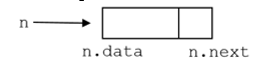
\includegraphics[width=0.25\paperwidth]{C:/Users/Admin/Desktop/Github/question_bank/LyX/static/img/9597-JPJC-2019-P2-Q8-1}
\par\end{center}

Complete the algorithm to implement the 'Delete' operation: \hfill{}{[}5{]}

\noindent %
\noindent\begin{minipage}[t]{1\columnwidth}%
\texttt{PROCEDURE Delete (x, i) }

\texttt{\qquad{}IF Length(x) = 0 THEN }

\texttt{\qquad{}\qquad{}....................................A.................................... }

\texttt{\qquad{}ENDIF }

\texttt{\qquad{}IF i = 1 THEN // situation 1: delete the 1st node }

\texttt{\qquad{}\qquad{}temp <- Start }

\texttt{\qquad{}\qquad{}....................................B.................................... }

\texttt{\qquad{}ELSE // situation 2 : delete middle node }

\texttt{\qquad{}\qquad{}Previous <- NULL }

\texttt{\qquad{}\qquad{}Current <- Start }

\texttt{\qquad{}\qquad{}FOR n <- 1 TO (i \textendash{} 1) STEP 1 }

\texttt{\qquad{}\qquad{}\qquad{}....................................C.................................... }

\texttt{\qquad{}\qquad{}\qquad{}....................................D.................................... }

\texttt{\qquad{}\qquad{}NEXT n }

\texttt{\qquad{}\qquad{}\qquad{}....................................E.................................... //
make the deletion }

\texttt{\qquad{}ENDIF }

\texttt{ENDPROCEDURE }%
\end{minipage}
\item Show how the following operations for an ADT called QUEUE using the
linked list ADT operations can be implemented. 
\begin{enumerate}
\item Create new queue. \hfill{}{[}1{]}
\item Add item to a queue. \hfill{}{[}2{]}
\item Delete item from a queue. \hfill{} {[}2{]}
\end{enumerate}
\end{enumerate}
{[}SPLIT\_HERE{]}
\item \textbf{{[}JPJC/PRELIM/9597/2019/P2/Q9{]} }

A binary search tree is stored as an array of records. Each record
represents a node and consists of the data and a left pointer and
a right pointer. After a number of records are inserted, the tree
is as shown. 

The array is called \texttt{BinaryTree}. 

The notation \texttt{BinaryTree{[}Root{]}.Data} will access the data
at root node.
\noindent \begin{center}
\begin{tabular}{c|c|c|c|}
\multicolumn{4}{c}{\texttt{BinaryTree}}\tabularnewline
\cline{2-4} \cline{3-4} \cline{4-4} 
 & \texttt{LeftPtr} & \texttt{DataValue} & \texttt{RightPtr}\tabularnewline
\cline{2-4} \cline{3-4} \cline{4-4} 
\texttt{{[}1{]}} & \texttt{2} & \texttt{Jay} & \texttt{3}\tabularnewline
\cline{2-4} \cline{3-4} \cline{4-4} 
\texttt{{[}2{]}} & \texttt{4} & \texttt{Gel} & \texttt{0}\tabularnewline
\cline{2-4} \cline{3-4} \cline{4-4} 
\texttt{{[}3{]}} & \texttt{0} & \texttt{Ken} & \texttt{5}\tabularnewline
\cline{2-4} \cline{3-4} \cline{4-4} 
\texttt{{[}4{]}} & \texttt{0} & \texttt{Ace} & \texttt{0}\tabularnewline
\cline{2-4} \cline{3-4} \cline{4-4} 
\texttt{{[}5{]}} & \texttt{6} & \texttt{Pan} & \texttt{0}\tabularnewline
\cline{2-4} \cline{3-4} \cline{4-4} 
\texttt{{[}6{]}} & \texttt{0} & \texttt{Max} & \texttt{0}\tabularnewline
\cline{2-4} \cline{3-4} \cline{4-4} 
\texttt{{[}7{]}} & \texttt{8} &  & \tabularnewline
\cline{2-4} \cline{3-4} \cline{4-4} 
\texttt{{[}8{]}} & \texttt{9} &  & \tabularnewline
\cline{2-4} \cline{3-4} \cline{4-4} 
\texttt{{[}9{]}} & \texttt{0} &  & \tabularnewline
\cline{2-4} \cline{3-4} \cline{4-4} 
\end{tabular}
\par\end{center}

\noindent \begin{center}
\texttt{}%
\begin{tabular}{c|c|c|c|}
\cline{2-2} \cline{4-4} 
\texttt{Root} & \texttt{1} & \texttt{NextFree} & \texttt{7}\tabularnewline
\cline{2-2} \cline{4-4} 
\end{tabular}\texttt{ }
\par\end{center}
\begin{enumerate}
\item Draw the binary search tree. \hfill{}{[}2{]}
\item Complete the algorithm to find a node in a binary search tree. This
function will return a pointer to node.\hfill{} {[}4{]}

\noindent %
\noindent\begin{minipage}[t]{1\columnwidth}%
\texttt{FUNCTION FindNode(SearchItem) RETURNS INTEGER }

\texttt{\qquad{}TempPtr <- Root }

\texttt{\qquad{}WHILE TempPtr <> NULL AND ............A............}

\texttt{\qquad{}\qquad{}IF ............B............ THEN }

\texttt{\qquad{}\qquad{}\qquad{}TempPtr <- BinaryTree{[}TempPtr{]}.LeftPtr }

\texttt{\qquad{}\qquad{}ELSE }

\texttt{\qquad{}\qquad{}\qquad{}............C............ }

\texttt{\qquad{}\qquad{}ENDIF }

\texttt{\qquad{}ENDWHILE }

\texttt{\qquad{}............D............}

\texttt{ENDFUNCTION} %
\end{minipage}
\item Write an algorithm for a pre-order traversal of the binary search
tree. \hfill{}{[}4{]}
\end{enumerate}
{[}SPLIT\_HERE{]}
\end{enumerate}

\end{document}
